\documentclass[10pt,a4paper]{article}
\usepackage[margin=1.7cm,top=1.5cm,bottom=1.7cm]{geometry}
\usepackage[T1]{fontenc}
\usepackage[utf8]{inputenc}
\usepackage{mathptmx}
\usepackage{courier}
\usepackage{microtype}
\usepackage{amsmath,amssymb,amsthm}
\usepackage{booktabs}
\usepackage{graphicx}
\usepackage{algorithm}
\usepackage[noend]{algpseudocode}
\usepackage{enumitem}
\usepackage{titlesec}
\usepackage[hidelinks]{hyperref}

\titleformat{\section}{\normalsize\bfseries}{\thesection.}{0.5em}{}
\titlespacing*{\section}{0pt}{0.8em}{0.3em}
\setlist{nosep,leftmargin=1.2em}
\setlength{\parskip}{0.25em}
\setlength{\parindent}{0pt}
\newtheorem{lemma}{Lemma}
\newcommand{\cost}{c}
\renewcommand{\algorithmicrequire}{\textbf{Input:}}
\renewcommand{\algorithmicensure}{\textbf{Output:}}

\begin{document}

\begin{center}
{\large\bfseries Budgeted, Dependency-Closed Context Selection for LLM Question Answering}\\[0.3em]
TC2038 Analysis and Design of Advanced Algorithms --- Midterm~1 (progress report) --- Equipo~5\\
Leandro Lizama Leirana (A00840242) \quad Rodolfo Aguirre Revilla (A00839754) \quad Andrés Maiztegui Martínez (A01833484)\\
Repository: \url{https://github.com/EQUIPO5/token-budget-selector} \quad October 2026
\end{center}

%-------------------------------------------------------------------------
\section{Problem, model and assumptions (Q1)}

\textbf{Resource problem.} An assistant that answers questions about a document normally sends the whole document as context, so the \emph{input tokens} consumed per query grow linearly with document length, whatever the question. Input tokens drive both monetary cost and latency. We therefore select a subset of the document that fits a token budget. Two difficulties make naive retrieval inadequate. First, documents repeat themselves, so the most relevant fragments are often paraphrases of one another. Second, some fragments are only correct together: an instruction sent without its exception yields a confidently wrong answer.

\textbf{Definitions.} The document is split into a finite set of \emph{fragments} $D=\{1,\dots,n\}$.
\begin{itemize}
\item $\cost_i\in\mathbb{Z}_{>0}$ is the \emph{cost} of fragment $i$: its length in tokens.
\item $B\in\mathbb{Z}_{>0}$ is the \emph{budget}: the maximum number of context tokens per query.
\item $r_i\in[0,1]$ is the \emph{relevance} of $i$ to the query $q$: the cosine similarity of their embeddings.
\item $s_{ij}\in[0,1]$ is the \emph{similarity} between fragments $i$ and $j$, with $s_{ii}=1$. Non-negativity is guaranteed because our embedding vectors have non-negative components.
\item $G=(D,E)$ is the \emph{dependency graph}. An undirected edge $\{i,j\}\in E$ means ``$i$ and $j$ are sent together or not at all''. A set $S\subseteq D$ is \emph{closed under $E$} if $\{i,j\}\in E$ and $i\in S$ imply $j\in S$.
\end{itemize}

\textbf{Inputs:} $(D, \cost, r, s, E, B)$. \textbf{Output:} a set $S\subseteq D$, sent to the LLM in document order.
\textbf{Constraints:} $\sum_{i\in S}\cost_i\le B$, and $S$ is closed under $E$.
\textbf{Objective:} maximise the \emph{relevance-weighted coverage}
\begin{equation}
f(S)=\sum_{i\in D} r_i\,\max_{j\in S} s_{ij},\qquad f(\varnothing)=0. \label{eq:f}
\end{equation}
Read term by term: every fragment $i$ of the document counts as ``represented'' by its most similar selected fragment $j$, to degree $s_{ij}$, and this is weighted by how relevant $i$ is to the query. A paraphrase of an already selected fragment adds little to $f$, because what it would represent is already represented. This is the \emph{facility-location} function~\cite{lin2011}. It is \emph{monotone} ($S\subseteq T\Rightarrow f(S)\le f(T)$) and \emph{submodular}: for $S\subseteq T$ and $x\notin T$, $f(S\cup\{x\})-f(S)\ge f(T\cup\{x\})-f(T)$. Both properties hold because each summand $\max_{j\in S}s_{ij}$ is a non-decreasing maximum of non-negative values, and non-negative weighted sums preserve them. Our tests check both properties numerically.

\textbf{Computational model.} The unit operation is the marginal-gain evaluation $f(S\cup b)-f(S)$, in the RAM model with real arithmetic. Embeddings, which are $d$-dimensional vectors, are given; producing them is the same preprocessing every retrieval system pays.

\textbf{Why this formulation.} The problem is NP-hard, since with $s$ equal to the identity matrix, $f(S)=\sum_{i\in S}r_i$ and it becomes 0--1 knapsack. An exact solution is therefore not a realistic goal, but submodularity gives a fast greedy algorithm with a proven constant-factor guarantee (Sec.~\ref{sec:alg}). We assume three things. (i)~Embedding similarity is a usable proxy for informational overlap. (ii)~Dependencies are known and symmetric; in practice they come from document structure, such as a clause and its sub-clauses, or from markers like ``except''/``unless'', and in the benchmark they are given. (iii)~Token count is the cost that matters. Assumption~(ii) is a deliberate simplification that we revisit in Sec.~\ref{sec:lim}.

%-------------------------------------------------------------------------
\section{Algorithm, invariants and correctness (Q2)}\label{sec:alg}

\textbf{Step 1: remove the closure constraint.} We contract the connected components of $G$ into \emph{blocks} using union-find, with cost $\cost_b=\sum_{i\in b}\cost_i$.

\begin{lemma}
$S$ is closed under $E$ if and only if $S$ is a union of connected components of $G$.
\end{lemma}
\begin{proof}
($\Leftarrow$) An edge never joins two different components. ($\Rightarrow$) If $i\in S$ and $j$ lies in the component of $i$, there is a path $i=v_0,\dots,v_k=j$. Closure gives $v_{t}\in S\Rightarrow v_{t+1}\in S$, so $j\in S$ by induction on $t$.
\end{proof}

Over blocks, $g(T)=f(\bigcup_{b\in T}b)$ is again monotone and submodular. The problem therefore becomes budgeted monotone submodular maximisation with no further constraint.

\textbf{Step 2: candidate pool.} We keep the most relevant \emph{whole} blocks until they contain at least $m$ fragments ($m=200$). This bounds all later work by $m$ rather than $n$ and preserves closure.

\textbf{Step 3: lazy cost-benefit greedy plus the best singleton} (Algorithm~\ref{alg}). Here $\Delta(b\mid S)=g(S\cup\{b\})-g(S)$ is the \emph{marginal gain} of block $b$. The \emph{stamp} records the size of $S$ at which a heap key was computed.

\begin{algorithm}[h]
\caption{\textsc{SelectContext}$(D,\cost,r,s,E,B,m)$}\label{alg}
\small
\begin{algorithmic}[1]
\State $\mathcal{B}\gets$ components of $(D,E)$ via union-find; keep the top blocks by $\max_{i\in b} r_i$ until $\ge m$ fragments
\State $S\gets\varnothing$; $R\gets B$; $t\gets 0$; $H\gets$ max-heap of $(\Delta(b\mid\varnothing)/\cost_b,\ b,\ \text{stamp}=0)$ for every $b$ with $\cost_b\le B$
\While{$H\neq\varnothing$}
  \State pop $(\kappa,b,\sigma)$ with the largest key $\kappa$
  \If{$\cost_b>R$} \textbf{continue} \Comment{$R$ never grows: $b$ can never fit again}
  \ElsIf{$\sigma=t$} \Comment{fresh key: by (I2) a true maximum}
     \If{$\kappa\le 0$} \textbf{break} \EndIf
     \State $S\gets S\cup b$;\ $R\gets R-\cost_b$;\ $t\gets t+1$
  \Else\ push $(\Delta(b\mid S)/\cost_b,\ b,\ t)$ \Comment{stale key: recompute it}
  \EndIf
\EndWhile
\State $b^\star\gets\arg\max_{b:\,\cost_b\le B} g(\{b\})$ \Comment{these values are already computed at line 2}
\State \Return $S$ if $g(S)\ge g(\{b^\star\})$, otherwise $b^\star$
\end{algorithmic}
\end{algorithm}

\textbf{Invariants.}
(I1)~After every iteration, $\sum_{i\in S}\cost_i\le B$ and $S$ is a union of blocks, hence closed under $E$ by the Lemma. This holds because a block is added only if $\cost_b\le R$.
(I2)~Every stored key is an upper bound on its block's \emph{current} ratio. A key is computed at some $S'\subseteq S$, and submodularity gives $\Delta(b\mid S)\le\Delta(b\mid S')$.
Consequently, when the popped key is fresh, it is at least every other stored key, and each of those is at least its block's true ratio, so the popped block is an exact argmax. Lazy evaluation (CELF~\cite{leskovec2007}) therefore returns \emph{the same set} as naive greedy, which recomputes every gain at every step. Our tests confirm identical values on 200 random instances.

\textbf{Optimality guarantee.} For monotone submodular $g$ with $g(\varnothing)=0$ under a knapsack constraint, the better of the cost-benefit greedy solution and the best single feasible element achieves $g\ge\frac12(1-\frac1e)\,\mathrm{OPT}\approx0.316\,\mathrm{OPT}$~\cite{khuller1999,krause2005}. The singleton branch is necessary. Without it, greedy can fill the budget with a cheap block of high ratio and then be unable to afford a large block worth arbitrarily more; a unit test exhibits this case.
\textbf{Algorithmic contribution.} The combination we propose is (a)~reducing dependency closure to block contraction, which preserves submodularity, (b)~using facility location to penalise redundancy, and (c)~CELF with the singleton rule for the budget. The result is a context selector with a certified worst-case ratio, whereas top-$k$ and MMR give no guarantee.

%-------------------------------------------------------------------------
\section{Complexity, guarantees and HPC (Q3)}

Notation: $n$ is the number of fragments, $d$ the embedding dimension, $m$ the pool size, $|E|$ the number of dependency edges, $\beta\le m$ the number of blocks in the pool, and $k$ the number of greedy additions.
\begin{itemize}
\item \emph{Per document (once):} embedding in $O(nL+nd)$, with $L$ the mean fragment length; union-find in $O(|E|\,\alpha(n))$, where $\alpha$ is the inverse Ackermann function.
\item \emph{Per query:} relevances in $O(nd)$; pool selection in $O(n\log n)$; pool similarities in $O(m^2d)$ time and $O(m^2)$ space; one gain evaluation costs $O(m\,|b|)$, so all initial gains cost $O(m^2)$.
\item \emph{Greedy loop:} in the worst case every key goes stale at every step, giving $O(k\,m^2)$ plus $O(\beta k\log\beta)$ for the heap, the same as naive greedy.
\end{itemize}
Total per query: $O(nd+n\log n+m^2d+km^2)$ time and $O(nd+m^2)$ space. Because $m$ is fixed, the cost is \emph{linear in $n$}. Without the pool ($m=n$) it would be $\Omega(n^2d)$.

Measured (median of 20 queries, single core): with $m=200$, query time grows from 7\,ms at $n=277$ to 43\,ms at $n=9015$, and selection itself stays at 2--3\,ms. Without the pool, time reaches 420\,ms already at $n=2243$ (Fig.~\ref{fig}, right). Laziness cuts gain evaluations by a factor of 3.7--5.3 relative to naive greedy, for example 366 against 1350 at $n=9015$.

\textbf{Exactness.} The algorithm is not exact; the proven bound is $0.316$. Empirically, on 300 pools small enough to solve by exhaustive search, the ratio $f(S)/\mathrm{OPT}$ has mean $0.988$, 5th percentile $0.926$ and minimum $0.868$; it equals the optimum in 61\% of cases, and the singleton branch wins in 7\%. Partial enumeration reaches $1-\frac1e$~\cite{sviridenko2004} but costs $O(\beta^5)$ gain evaluations, which these numbers do not justify.

\textbf{HPC.} We do not use HPC, for a measurable reason. Selection (2--3\,ms) is a sequential chain of dependent greedy steps, while the parallelisable part is the $O(nd)$ relevance product together with the $O(m^2d)$ similarity block. If those are row-partitioned across $p$ workers, each worker computes $O(nd/p)$. Communication consists of broadcasting $q$ ($d$ values) and gathering $p$ local top-$m$ lists ($O(pm)$ values). Parallel efficiency is therefore near~1 only when $nd/p\gg d+pm$, that is, for documents far larger than our workloads. By Amdahl's law the sequential selection bounds the achievable speed-up per query at roughly $43/3\approx14\times$. Batching many queries is the better use of parallel hardware.

%-------------------------------------------------------------------------
\section{Evaluation protocol and preliminary results (Q4)}

\textbf{Workloads.} We use a synthetic benchmark with known ground truth (\texttt{tokenopt/synthetic.py}). Each topic contributes a rule, an exception with probability~0.6 (linked to its rule by a dependency edge), 0--4 near-duplicates of the rule (median similarity 0.88), and two noise fragments. A query about topic $t$ has the gold set \{rule, exception\}. To increase the workload we vary $n$ from 277 to 9015 fragments; to tighten the resource constraint we vary $B\in\{150,300,600\}$ tokens.

\textbf{Alternatives.} We compare against three baselines: (i)~\emph{full context}, the unoptimised baseline; (ii)~\emph{top-$k$}, which adds the most relevant fragments while they fit; and (iii)~\emph{MMR}~\cite{carbonell1998} with $\lambda=0.7$, the standard diversity heuristic. All methods share the same pool and similarities.

\textbf{Metrics.}
\begin{itemize}
\item \emph{Resource consumption:} input tokens and latency.
\item \emph{Completeness:} the percentage of queries whose whole gold set is sent.
\item \emph{Correctness proxy:} the percentage of queries in which some dependency is broken, meaning an instruction is sent without its exception or vice versa.
\item \emph{Redundancy:} the share of selected tokens spent on a second or later copy of the same content.
\item \emph{Consistency:} whether the selected set is identical across reruns and across permutations of fragment order.
\end{itemize}

\textbf{Reproducibility.} Five corpus seeds with 60 queries each; every random generator is seeded; the embedding is deterministic; results are reported as mean $\pm$ standard deviation across seeds. A single script, \texttt{experiments/run.py}, produces every number in this document.

\begin{table}[h]\centering\small
\begin{tabular}{@{}llrrrr@{}}
\toprule
$B$ & method & tokens sent & complete (\%) & broken dep.\ (\%) & redundant tokens (\%)\\
\midrule
--  & full context & $13384$ & $100$ & $0$ & $39.7$\\
\midrule
150 & top-$k$ & $143$ & $56.7\pm3.9$ & $41.0\pm2.7$ & $36.0$\\
    & MMR     & $143$ & $35.7\pm4.3$ & $53.7\pm8.7$ & $6.5$\\
    & \textbf{ours} & $136$ & $55.7\pm3.7$ & $\mathbf{0}$ & $10.6$\\
\midrule
300 & top-$k$ & $293$ & $86.3\pm2.9$ & $46.7\pm13.4$ & $36.2$\\
    & MMR     & $293$ & $46.3\pm0.7$ & $77.7\pm5.0$ & $7.4$\\
    & \textbf{ours} & $257$ & $\mathbf{88.3\pm2.4}$ & $\mathbf{0}$ & $23.2$\\
\midrule
600 & top-$k$ & $593$ & $94.0\pm2.0$ & $71.0\pm17.7$ & $25.8$\\
    & MMR     & $594$ & $50.0\pm1.1$ & $98.0\pm1.9$ & $4.2$\\
    & \textbf{ours} & $\mathbf{406}$ & $\mathbf{97.7\pm0.8}$ & $\mathbf{0}$ & $30.3$\\
\bottomrule
\end{tabular}
\caption{Preliminary results (5 seeds $\times$ 60 queries). Full context is complete by construction, but it spends 23--98$\times$ more tokens than any budgeted method.}\label{tab}
\end{table}

\begin{figure}[h]\centering
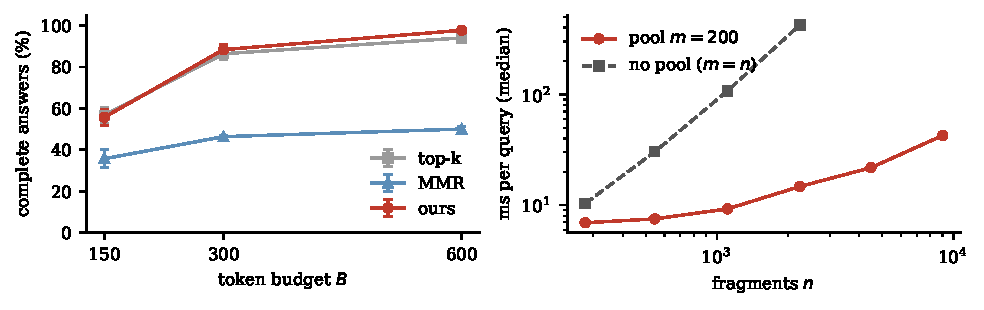
\includegraphics[width=0.8\linewidth]{fig.pdf}
\caption{Left: completeness against budget. Right: median time per query against document size, log--log scale.}\label{fig}
\end{figure}

\textbf{Reading the results.} At equal budget our method matches or beats top-$k$ in completeness and \emph{never} breaks a dependency, whereas top-$k$ breaks at least one in 41--71\% of queries and MMR in 54--98\%. At $B=600$ it reaches the highest completeness while using 32\% fewer tokens, because it stops once no remaining block adds positive coverage. MMR is the least redundant method, but it is also the least complete: it diversifies \emph{away} from the exceptions. Selections are identical across reruns. Under permutations of fragment order, 95.3\% of selections are identical (mean Jaccard similarity 0.991); the differences come only from ties broken by fragment index.

\textbf{Next stage.} We will feed the same contexts to a fixed LLM at temperature~0, score its answers against reference answers for correctness, count tokens with that model's own tokenizer, and repeat runs to measure answer consistency, all on a real document collection.

%-------------------------------------------------------------------------
\section{Limitations and prioritised improvements (Q5)}\label{sec:lim}

\textbf{Limitations.}
(L1)~Dependencies must be known and are treated as symmetric. A directed relation, where an exception needs its rule but a rule does not need its exception, is forced into one block, which over-spends tokens.
(L2)~Leftover budget is spent on near-duplicates: 23--30\% of tokens at $B\ge300$ (Table~\ref{tab}).
(L3)~Relevance is lexical (hashed TF-IDF), and completeness is a proxy for answer quality.
(L4)~The guarantee of $0.316$ is loose in comparison with what we observe.
(L5)~Ties are broken by fragment index, which costs 4.7\% of permutation-consistency.

\textbf{Improvements, in priority order.}
\begin{enumerate}
\item \emph{Duplicate clustering with edge inheritance} (addresses L2). Before selection, cluster fragments with $s_{ij}\ge\tau$ and keep one canonical representative that inherits \emph{every} dependency edge of its cluster. A pilot run motivates the inheritance step: simply setting $s_{ij}=1$ above $\tau$ \emph{lowered} completeness at $B=300$ from 88.3\% to 84.0\% ($\tau=0.85$) and to 69.3\% ($\tau=0.75$), because a paraphrase displaced the rule that the exception is attached to. Expected benefit: redundant tokens close to 0 at unchanged completeness. Evaluation: completeness and redundancy as functions of $\tau$, on the same five seeds.
\item \emph{Directed dependencies} (addresses L1). Model $E$ as a DAG and select \emph{closures}: the cost of choosing $i$ becomes the cost of $i$ plus its not-yet-selected ancestors, so the problem becomes precedence-constrained knapsack. Expected benefit: fewer tokens at equal completeness on documents whose exceptions are optional. Evaluation: a variant of the benchmark with directed edges, reporting tokens at a fixed completeness, against the current undirected version.
\item \emph{Semantic relevance and end-to-end scoring} (addresses L3 and L5). Replace the embedding with a sentence-embedding model and break ties by a content hash, which makes the result invariant to fragment order. Expected benefit: better recall on paraphrased queries and 100\% permutation-consistency. Evaluation: the end-to-end LLM protocol of Sec.~4 at temperature~0, under fixed seeds and a fixed model version.
\end{enumerate}

\vspace{-0.4em}
{\footnotesize
\begin{thebibliography}{9}\setlength{\itemsep}{0pt}
\bibitem{carbonell1998} J.~Carbonell, J.~Goldstein. The use of MMR, diversity-based reranking for reordering documents and producing summaries. \emph{SIGIR}, 1998.
\bibitem{khuller1999} S.~Khuller, A.~Moss, J.~Naor. The budgeted maximum coverage problem. \emph{Inf.\ Process.\ Lett.} 70(1):39--45, 1999.
\bibitem{krause2005} A.~Krause, C.~Guestrin. A note on the budgeted maximization of submodular functions. Tech.\ Rep.\ CMU-CALD-05-103, 2005.
\bibitem{leskovec2007} J.~Leskovec et al. Cost-effective outbreak detection in networks. \emph{KDD}, 2007.
\bibitem{lin2011} H.~Lin, J.~Bilmes. A class of submodular functions for document summarization. \emph{ACL}, 2011.
\bibitem{sviridenko2004} M.~Sviridenko. A note on maximizing a submodular set function subject to a knapsack constraint. \emph{Oper.\ Res.\ Lett.} 32(1):41--43, 2004.
\end{thebibliography}}

\end{document}
